\documentclass[a5paper]{article}
\usepackage[utf8]{inputenc}
\usepackage[russian]{babel}
\usepackage{lmodern}
\usepackage{url}
%\usepackage{pscyr}
\usepackage[svgnames]{xcolor}
\usepackage{pdfcolmk}
\usepackage{graphicx}
\usepackage{tikz}
\usepackage{pifont}
\newlength{\drop}
\usepackage{geometry}
\newcommand*{\titleTMB}{\begingroup% Three Men in a Boat
\drop=0.1\textheight
\centering
\settowidth{\unitlength}{\LARGE THE BOOK OF CONUNDRUMS}
\vspace*{\baselineskip}
{\HUGE\scshape АС}\\[\baselineskip]
\rule{\unitlength}{1.6pt}\vspace*{-\baselineskip}\vspace*{2pt}
\rule{\unitlength}{0.4pt}\\[\baselineskip]
{\HUGE \textbf{Мы \\ --- \\
Осколки}}\\[\baselineskip]
%59{\itshape puzzles for the mind}\\[0.2\baselineskip]
\rule{\unitlength}{0.4pt}\vspace*{-\baselineskip}\vspace{3.2pt}
\rule{\unitlength}{1.6pt}\\[\baselineskip]
\vfill
\endgroup}

\author{АС}
\title{Мы --- Осколки}
\usepackage{pdfpages}

\begin{document}
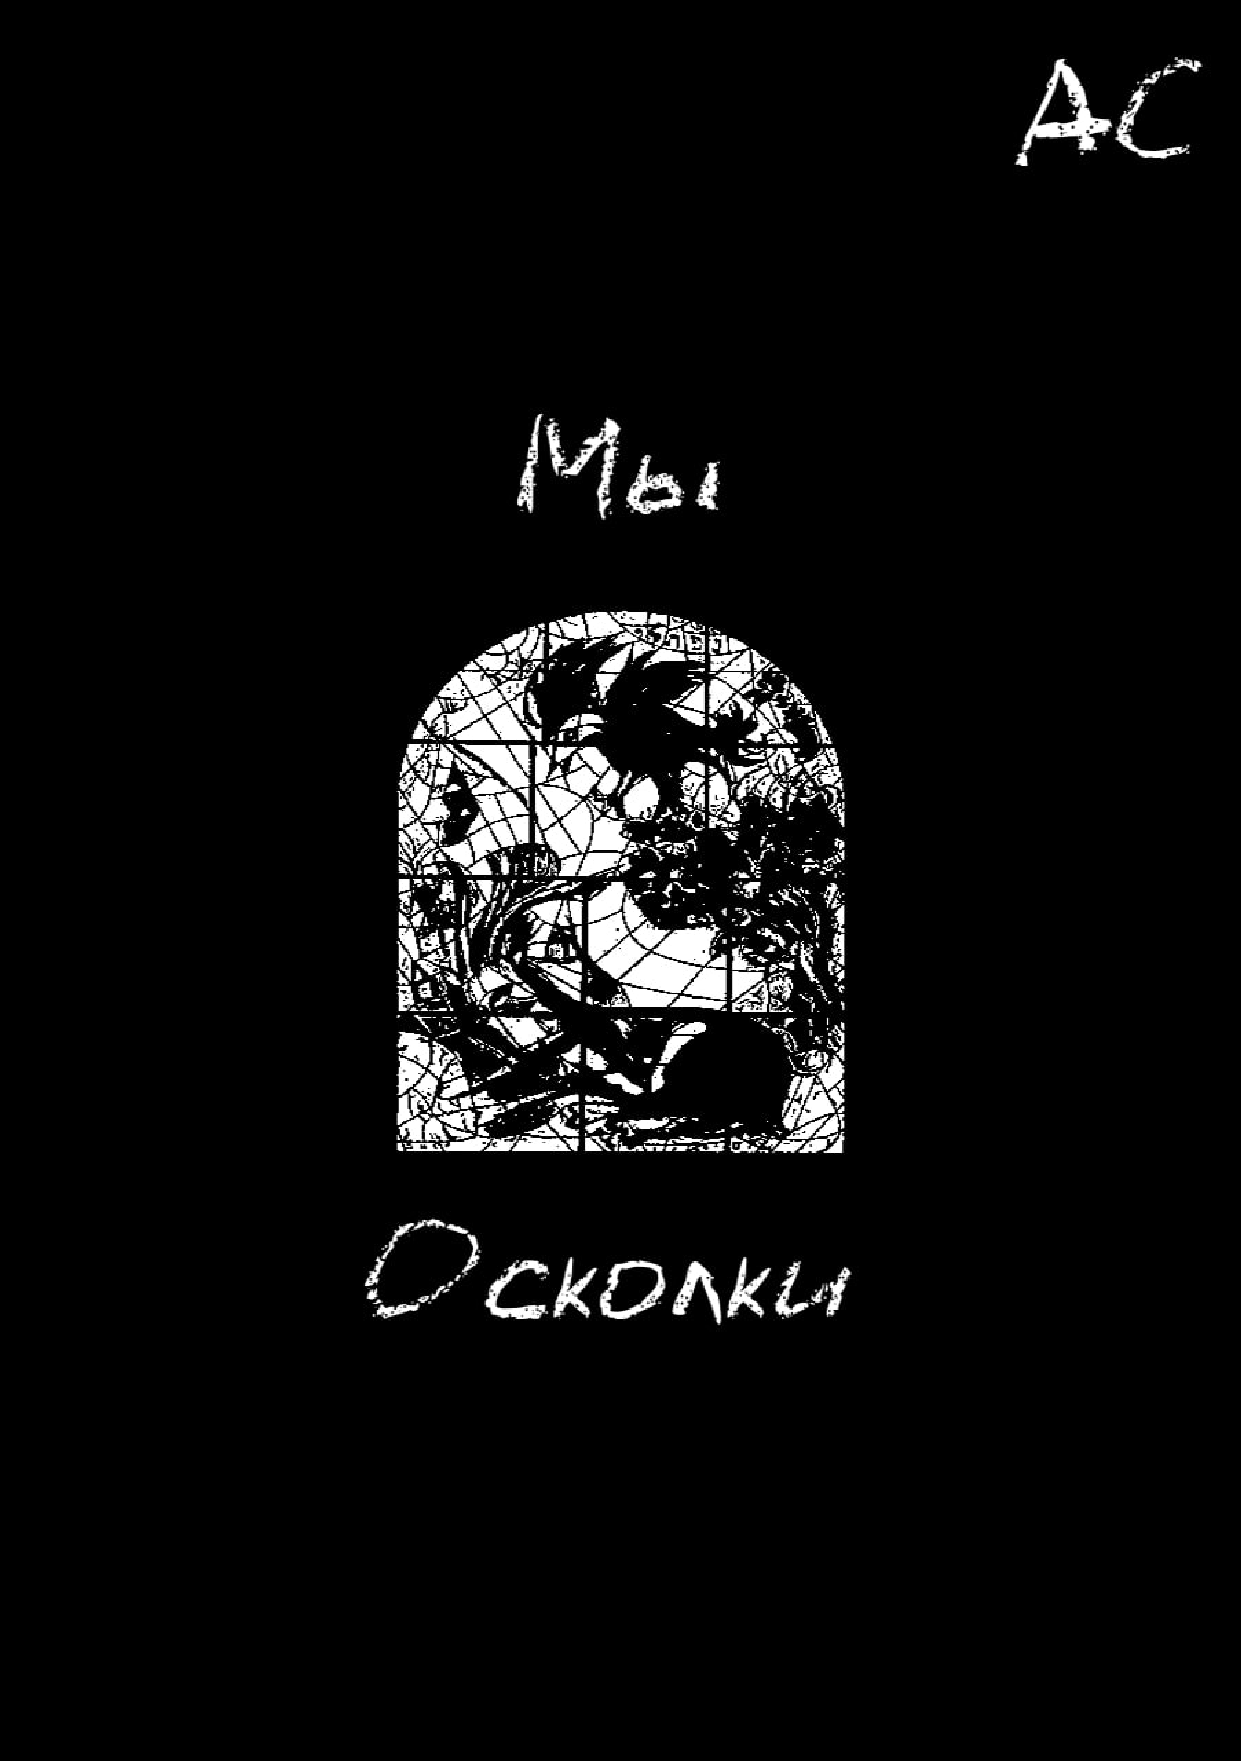
\includepdf{cover.pdf}

\pagenumbering{gobble}% Remove page numbers (and reset to 1)


Мы --- Осколки

А.С.

Ты обманывал нас, обезумевший Фриц, ---Бог не умер, он просто так пахнет...

М.Успенский. Райская Машина

\section{1}

...-- Понимаешь, мы --- никто!

Она кричит.

Нет, ей даже не тяжело. Это не истерика, это скорее экспозиция. Заявка на главные темы, акценты, сюжетные линии и переходы... А сейчас, уважаемая публика, вы прослушаете легкое аллегро в струнном исполнении.

-- Господи, какой же ты идиот! Неужели ты не видишь этого? От нас ничего не осталось!

Она смеется, и ее смех упруго отражается от забитых слабоподсвеченных стен и плотно закрытого окна.

Она сидит на краю стола, свесив босые ноги на пол, покручивая в нервных, тонких, обтянутых хрупкой, словно оберточная бумага, кожей ладонях тяжелый стакан с водкой. На ней непонятное серое платье, больше похожее на ночную сорочку, пожалуй, чересчур честно прилегающее к ее фигуре. Но сейчас ей на это плевать.

Сейчас она --- голос.

-- Ты же чувствуешь это, да? Мы подножный корм! Можешь сколько угодно обманывать себя и других, но ты чувствуешь это! Отыгранная, безынтересная падаль, отражающаяся в зрачках собеседника. Ты же боишься меня сейчас?

Стакан пустеет. Боюсь.

-- Ты боишься, ведь я --- правда.

У нее горят глаза. В ней не осталось ничего тонкого, изящного, что обычно ищут в красивой женщине. Не осталось недоведенных взмахов рук, недосказанных фраз. Сейчас она --- от начала и до конца, без поблажек. Сейчас она говорит все, не жалея ни себя, ни меня; сейчас она вкладывает все в каждый взмах руки, в каждое слово, в каждую эмоцию.

Она --- голос.

-- Просто скажи это. Не смей мне врать. Неужели тебя не тошнит от каждого, кто осмелился назвать себя человеком?

Неосторожное движение --- и стакан отправляется на пол. В звенящей тишине он крошится об пол практически беззвучно --- композиция из затемненного стекла, плавно превращающегося в калейдоскопную крошку, растекающуюся по неровному полу. Она смеется:

-- Вот они, мы. Уродливая стекольная пыль. Хочешь, делай вид, что каждый способен блестеть...

Она делает глоток прямо из бутылки, яростным кивком отбрасывает волосы назад.

-- Думаешь, это красиво?..

Да, красиво.

-- Но на деле ты уже на полпути к мусорному ведру.

\section*{2}

В детстве ей очень нравились глиняные и стеклянные черепки, остающиеся от разбитой посуды. Она никак не могла понять, почему люди такие глупые и выкидывают их, эти несчастные останки кухонной утвари. Мама тоже была глупая, но с ней можно было договориться за сделанные уроки. Тогда мама ворчала весь вечер, но уговор соблюдала, оставляя ей осколки.

Они были красивые, но всегда обычные.

Необычные иногда появлялись на улице, когда какая-нибудь семья, устав врать друг другу, громко взрывалась на всю округу неприятными подробностями. Подробности ей не очень нравились, тем более, что они всегда были одинаковыми, а вот черепки выкинутой в окно посуды всегда были разными. Некоторые из них были покрыты разноцветной эмалью, но так ярко сверкали на солнце, что живущие на той же улице мальчишки хватали их первыми и уже не отдавали. Ругаться с ними ей не хотелось, а меняться с мальчишками было не на что, так что разноцветных всегда не хватало.

Она приносила добычу домой, долго отмывала ее в заранее набранном ведерке с водой и ласково укладывала в коробку под кроватью. В дни же, когда ей становилось грустно, она вытаскивала свои сокровища на свет и перебирала их, постоянно обрезаясь об острые края. Иногда она выбрасывала всех их на пол и пыталась сложить из них картинку.

Глупая мама заходила в комнату, заглядывала через плечо и спрашивала: что это? Тогда она вздрагивала, оборачивалась и поднимала на маму полные недоумения глаза:

-- Это мы, мамочка. Как же ты не понимаешь?

Мама действительно не понимала, но признаться в этом ей не хватало духу, и она уходила. Пройдет время, думала мама, картинка получится, и ее девочка наконец повзрослеет.

Картинка никогда не получалась, и она знала почему: ей не хватало черепков. Тогда она собирала всех подопечных обратно, забиралась на чердак и смотрела на небо, оставив разочаровавшие ее сокровища внизу.

Она знала, что время этих осколков еще не пришло.

Потом в Городе началась Война. Ей нравилось писать это слово именно так, с большой буквы. Взрослые в школе ругались, мазали тетрадку красными чернилами и сердито смахивали назойливую заглавную В с меловой доски. Но ей всегда казалось, что эта одна разъединственная буква заставляет их всех выпрямлять спину, и она снова ее писала, довольная своей маленькой магией.

Война превратила улицы в целые галереи черепков, где, казалось, можно было найти любой осколочек, у которого был хоть малейший шанс появиться на земле. Она ходила по этим галереям, как завсегдатай музея, вдобавок объехавший все самые важные мировые выставки, и грустила. Ей казалось, что вот сейчас она точно сможет собрать картинку, но обнаружилось, что Война оставляет после себя самые обычные увечные черепки, и ничего кроме них.

И не было никакой разницы, сидел ли на этой улице подлый враг, который раньше, как известно из одного странного, но понравившегося ей рассказика, обретался где-то за лесом, или здесь защищались наши доблестные войска --- вместо них остались одинаковые осколки, непригодные ни для чего, кроме печальных воспоминаний о произошедшем.

Но однажды Война сделала ей подарок: почти отсыревший заряд попал в крышу собора в еще нетронутой части Города и взорвался внутри, выбив витражные стекла. Кто-то закричал, какие-то проходившие мимо люди плакали от бессилия, наблюдая, как рушится под собственным весом то, что они считали святым. А она стояла под чудесным цветным стеклянным облаком, опасными иголками оседающим на тротуар, и смеялась. Прохожие в ужасе смотрели на нее, отчаянно пыталась пробиться к ней через толпу перепуганная мама, а она танцевала под великолепным витражным вихрем, ощущая, как горячими стеклянными каплями пополам с кровью сбегают по ней новые, подаренные Войной, фрагменты ее картинки.

Нас.

И тогда она решила, что нужно только ждать, пока мозаика на полу ее спальни сама не соберется в ее руках. Пока не настанет время...

\section*{3}

... -- Знаешь, что я усвоил за все это время, Мишка?

Череда переулков иногда прерывалась сериями сквозных подвалов, в которых чадили керосиновые лампы и пахло махоркой, которую в Городе в последнее время выращивали даже на подоконниках. Старик тащил его этой дорогой с невозможной скоростью, так, что практически приходилось перепрыгивать через бездомных, уютно устроившихся в этих лабиринтах Нижнего Города. Бездомные, впрочем, особо не возражали --- в конце концов, свои...

-- Все настоящее, Мишка, случается не по плану.

На старике замызганная длинная кожанная куртка, давшая носителю прозвище, пропылившаяся и выгоревшая на солнце настолько, что хотелось отнести ее в музей. Впрочем, ее хозяина тоже вполне можно было бы определить туда же --- жители Нижнего Города даже шутить боялись по поводу его возраста.

-- Понимаешь, абсолютно все! Никто не планировал, что я проживу столько --- но вот он я, черт возьми... Да и тебя, одиночку, списали в крысиный корм. Как только ты решил, что вот так будет дальше --- все, настоящее закончилось.

Несколько полуснесенных Войной зданий, заваленный кирпичами переулок, длинная лестница в новый виток Нижнего Города. Мишка неплохо ориентировался здесь, но понятия не имел, куда тащит его Куртка, бодро шагающий впереди.

-- Жалко мне их. Представляешь, они планируют жизнь. Знают наперед, когда сменят работу, когда легкое касание рук перейдет в поцелуй, когда появятся дети. Они придумывают себе реальность! Без вкуса, цвета и запаха, известную до каждого чиха... И умудряются в ней жить. В никакой. Ненастоящей.

-- Так проще.

Куртка оборачивается, вглядываясь в мишкино лицо. Только тогда он замечается, что старик улыбается.

-- Нет, Мишка. Ничуть не проще. Просто не так страшно. Человек очень сильно боится смотреть в глаза себе и другим, не надев очки. Почти пришли...

Старик подхватил догорающую лампу и устремился в угол очередного подвала, где обнаружилась небольшая, метра полтора в высоту, дверь, за которой по отсветам угадывалась винтовая лестница. Преодолев ее, старик отбросил крышку люка в полу и неожиданно сильной рукой помог выбраться из хода своему спутнику.

Дом, в котором они оказались, пострадал от Войны не так заметно, как многие другие в этой части Города. Несколько снарядов пробило крышу и взорвалось внутри того зала, куда Куртка привел своего товарища. Окна в комнате были выбиты, несколько столов и шкафов раскурочены взрывами, пол усыпан бумагами, большая часть из которых вряд ли пережила пожар после бомбежки. В углу почти разрушенной стены торчал самый обыкновенный пишущий телеграф, словно в насмешку оставшийся в целости.

-- Добро пожаловать в Рубку, -- пробормотал Куртка, пустым взглядом обводя комнату.

Мишка скользил между столов, заглядывая в разбросанные бумаги. Планы города, приказы о мобилизации, схемы отступления... Здесь началась Война. Та самая, которая всю его жизнь яростно скалилась ему в лицо. Та самая, которая танцевала сейчас на улицах города уже привычной, прижившейся актрисой передвижного и довольно жестокого театра.

Ноги сами понесли его к телеграфу. Бумажная лента была на месте, хотя должна была бы сгореть.

подлый враг среди нас тчк северсевервосток тчк уничтожить

-- Куртка!..

Голос осип.

-- Это же ведь он, да? Приказ о первом ударе?..

Старик мягко улыбнулся и направился к телеграфу.

-- Думаешь, это самое страшное в этой комнате, Мишка?

Он пересек комнату и обогнул остаток стены, у которой стояло устройство связи.

Телеграфная линия аккуратно уходила в стену и выходила с другой стороны, чего, видимо, нельзя было заметить до её разрушения.

Провода были спаяны и опломбированы.

-- Самое страшное --- вот!

... На пломбе стояла дата постройки здания.

\section*{4}

Времен года в Городе почти не осталось. Так, теплая осень, холодная осень... Да и то без всякой разумной системы. Зато всегда был ветер, словно пытающийся выдуть несчастные остатки людей, безмозгло цепляющиеся за свои дома.

Запаха у ветра было всего два. Чаще всего он пах ближайшим пожаром, рожденным новой серией снарядов, пущенных уже и неизвестно с чьей стороны. Такой ветер был жестким; он обдирал горло и забирался поглубже в легкие так, чтобы каждый долго и мучительно откашливался, заставляя жителей выбираться на улицу с обязательной марлевой повязкой в кармане. Иногда ветер пах дождем, жадно льющимся в одной из частей Города. Когда выдавались такие дни, люди выбирались наружу, втягивая в себя озонированный воздух, как будто пытались надышаться вперед. И Война замирала, щедро раздаривая время всем, кто мог его оценить.

Последний дождь закончился полчаса назад. На заросшем пустыре, предваряющим вход в школьный двор, стоял съежившийся человек средних лет, замотанный в длинное пальто, как в герметичную упаковку. Человек буравил взглядом блок бетонного забора, щедро выкрашенный белой краской, и уже двадцать минут не мог отвести взгляд.

...Они, мальчишки, называли его Форум, как место для народных собраний во времена Древнего Рима.

Во времена начальных классов на Форуме царил раздрай и полная свобода --- его неудачливую поверхность бороздили десятки надписей, сделанные ребятами; причем надписи довольно редко были сколько-нибудь цензурными и превышали по длине три заповедные буквы. Пару раз забор переживал катастрофы в виде школьного сторожа с ведром краски, но вскоре снова возвращался в привычное скабрезное состояние.

Потом в Городе началась Война, и Форум изменился.

Сначала мальчишки бредили боями на фронте, предрассветными арт-подготовками, безупречным мужеством и героическим отчаянием, которыми за километр несло от картонных героев военных книжек и газетных репортажей. Все глупости на Форуме были решительно закрашены, а поверх них были выведено черной краской:

Мы не сдадимся!

Никто и не думал сдаваться, но шло время, а Война все продолжала звенеть над Городом теперь уже единственным полифоническим оркестром, упрямо обходя стороной школу и авторов Форума. В голову им забредали изящные картинки военных парадов, с которых отправлялись сразу на передовую, безмозглых тыловых балов времен империи, когда раненые офицеры танцевали с красивыми дамами, потягивая вино. Надпись на Форуме уступила место для многообещающего, но необъяснимо пугающего:

Скоро наш черед!

Черед в итоге настал, и в школу ночью попало два снаряда, разворотивших верхние этажи. Первый раз увидев заглянувшую к ним на огонек Войну, они, удивленные, бродили между разбитых осколками кабинетов, подбирая разбросанные учебники и выкручивая лампочки, чтобы отнести их все в подвал, где с этого момента проводились основные занятия. Они знали теперь, что Война среди них; им казалось, что они уходят в подполье, чтобы пускать вражеские поезда под откос, в темноте выбираясь из подвалов и схронов. Теперь на заборе красовалось:

До последнего вздоха!

Потом кто-то из них погиб под завалами около своего дома, у кого-то еще завербованный в первые месяцы отец не вернулся домой. Они стали достаточно взрослыми, чтобы замечать, как бегут из-под обстрела наши доблестные войска; как прячутся по кладовкам дезертиры; как оставшиеся без крыши и денег дерутся за кусок пайка и убивают друг друга в драке. Они стали достаточно зрячими, чтобы за лоском и шумом газетных статей и траурных песен видеть настоящую Войну. Ту, где единственным постоянным желанием является обеих сторон является лишь одно --- выжить, выжить через всю грязь и кровь, кислотой сочащиеся вокруг. Ту, где враг не так уж подлее друга, а друг не слишком честнее врага. Обезумев от этого зрелища, они написали на Форуме одно слово:

Хватит!

Впрочем, они знали, что это ничего не изменит. Эта надпись нужна была им самим, каждому в отдельности, как точка отсчета, чтобы знать, что ты уже точно сказал нет. Пусть даже этого никто и не услышал, кроме тебя самого.

Война продолжала жить рядом с ними, исправляя эту самую жизнь по своему усмотрению. Война забирала их любимых, меняла маршруты прогулок, решала за них квартирный вопрос --- фактически, Война воспитывала их заново, словно разрешая сделать одно, заставляя выбрать другое и оставаясь равнодушной к третьему.

Через двадцать лет они пришли к Форуму, чтобы нанести новую надпись. Они жили в Войне. Их дети родились в ней и воспитывались ею на тех же правах, на каких их воспитывали родители. Она не просто стала частью их жизни --- она стала нормальной её частью. Все те грязь и кровь, кислотой сочащиеся вокруг, никуда не исчезли, а впитались в воздух и стали новой приправой к приевшемуся кислороду...

Человек средних лет улыбнулся, глядя на кипельно белый Форум.

Два года назад они собирались написать здесь Нам плевать, но только закрасили старую надпись и разошлись.

Потому что те, кому действительно плевать, не пишут об этом на заборах.

\section*{5}

...Новая череда подвалов.

Говорят, Город был пронизан ими еще до начала Войны, но только после они стали сквозными.

Куртка сжалился над Мишкой и сбавил темп. А возможно, этому поспособствовала бутылка дешевой трактирной бражки, украденная ими сегодня с утра и опустевшая в руках бездомных уже наполовину.

Чудное дело --- алкоголь словно пролетал мимо головы, не производя никакого эффекта, если не считать того, что Мишку уже пару раз выворачивало, да и то скорее всего от нервов. Говорить особо не хотелось, да и Куртка запретил, жестко оборвав на выходе из Рубки:

-- Ни слова, пока не дойдем еще до одного места.

И они шли. Пили и шли, как подобает любому приличному путешествию.

Здесь, “ниже уровня моря”, жизнь шла своим чередом: люди обустраивали дома, делили участки подвалов, чтобы выгадать поближе к выходу, где обязательно находилась система самопальных огородов. В большинстве коридоров дышать было сложно из-за табачного дыма; кое-где раздавался детский плач.

Казалось, все это может сойти за самый обычный город, но хватало одного взгляда на лица живущих здесь, чтобы понять, что эта никакая не обычная жизнь. Сюда приходили переночевать те, кому некуда было больше идти. Приходили --- и с утра уходили снова, на неспокойный верх, где осталась жизнь прежняя. Здесь вообще не было принято грустить по тем, кто не возвращался.

Живой осел лучше дохлого льва --- это правда; как правда и то, что живым себя можно считать при весьма определенных условиях.

Ощущения слегка притупились бражкой, но судя по всему спутники двигались в противоположном прежнему направлении. Куртка терпеливо молчал, уверенно выбирая повороты; дышал старик, казалось, даже умиротворенно, словно у него вошло в привычку каждый день проходить в исключительно бодром темпе пару десятков километров по пересеченной местности.

Наконец он снова подхватил лампу, осветив темный угол очередного подвала, отбросил какие-то картонки и обнаружил за ними очередную карликовую дверь с винтовой лестницей.

Из люка на этот раз Мишка выбрался сам, без особого удивления оказавшись в комнате, почти совпадающей с только что покинутой ими Рубкой. Главным отличием было лишь то, что здесь огонь постарался на славу, сожрав почти все бумаги и мебель.

В углу все такой же насмешкой громоздился телеграф.

Мишка обернулся, чтобы посмотреть на своего спутника. Куртка стоял в противоположном углу комнаты, скручивая из запасенной махорки сигарету. Старик поймал взгляд и кивнул в направлении телеграфа.

Стена пострадала от обстрела гораздо меньше, чем в первой Рубке, так что Мишке пришлось взбираться на стол, на котором стояло устройство связи, чтобы разглядеть линию.

Линия ничем от увиденной ими раньше не отличалась --- она все так же вела в никуда, заканчиваясь нетронутой пломбой, поставленной задолго до начала Войны.

Куртка засунул так и не подожженную сигарету в карман, пересек комнату и взял в руки телеграфную ленту.

-- Что забавно, обе не сгорели, представляешь?..

На ленте, подпаленной с конца, гордо значилось:

подлый враг среди нас тчк югюгзапад тчк уничтожить

\section*{6}

... -- Ты трус.

Она лежит рядом, рассыпав свои словно выгоревшие волосы по моему плечу.

-- Ты самый настоящий трус. Ты так боишься жестких ответов! Наверное, может быть... Засунь себе это знаешь куда? Бывает только так, а не иначе! Ты слышишь --- только!

Самое смешное, что она даже не повышает голоса, выговаривая все это шепотом. Так обычно бывает после шторма, когда кажется, что любое неосторожное слово может сломать воцарившуюся хрупкую тишину.

-- Тебе хочется всегда иметь запасной выход. Хочется знать, что любую стену можно пробить, любое нет можно повернуть в да, что никогда не бывает ничего наверняка. И поэтому ты не можешь признать, что я права; думаешь, что я заблуждаюсь, что я, как последняя дура, обманываю себя...

Думаю.

Хотя какая сейчас разница.

-- Всегда есть разница.

Ей не нужно кричать --- слова вспарывают тишину и вонзаются в уши, как гвозди в ладони, оставляя за собой слишком много боли.

-- Тебе хочется думать, что человеческие чувства, человеческие поступки ничем не отличаются от задачек по физике. Тебе кажется, что если я всегда могу ошибиться, вычерчивая силы мелом на доске, то и здесь я всегда могу оказаться не права. Что нет никаких гарантий...

Ее кожа на ощупь похожа теплую глину, только вышедшую из под пальцев гончара: кажется, что сейчас ты можешь сделать все, что захочешь, но на деле игра уже закончена, и результат известен. Весь вопрос в том, сможешь ли ты с ним смириться?..

-- Тебе кажется, что все это --- просто вопрос веры. Я верю, что все происходит именно так, а не иначе. Что все это может опровергнуть кучка ученых, высадившись на каком-нибудь изолированном острове. Что это всего лишь мое собственное евангелие...

Какой же жестокий бог в этом евангелии!

Евангелии имени тебя.

Она соскальзывает с плеча, кровати и медленно направляется в противоположный угол комнаты.

-- Но ты просто трус. Ты боишься того, что я права. Дай тебе крохотную надежду --- и ты будешь жить ей, дышать ей, пока ожидание невозможного не вгонит тебя в запой. Ты так и будешь надеяться выиграть в этой гонке за чудом, вместо того, чтобы принять правду и жить с ней...

Только вот кто сказал, что это правда?

-- Каждый выбрал ее себе сам. И только ты предпочел ничего не выбирать.

Она вытаскивает из под шкафа довольно большую картонную коробку. Коробка празднично позвякивает.

...в город завезли фальшивые елочные игрушки. Они такие же, как настоящие, только радости от них никакой...

\section*{7}

...-- Это же ведь подделка, да?

Они покидают Рубку так же быстро, сбрасывая темп только районе центра Нижнего Города.

-- Куртка, ты же понимаешь, что это всего лишь подделка?

Со стороны может показаться, что Мишка практически спокоен. Лишь только два горящих ярким огнем глаза выдают то безумие, что творится у него внутри.

Куртка выбрасывает опустевшую бутылку и внимательно смотрит на молодого человека:

-- А есть ли разница?

В ответ Мишка упоенно трясет головой, как делают собаки, выбравшись из воды.

-- Что ты несешь, конечно есть. Если это не подделка, то эти две Рубки могут остановить Войну...

Бездомные не обращают на них никакого внимания. Казалось бы, подобная фраза должна вызвать хоть какую-то реакцию, но в ответ поднимает голову только маленькая девочка, заснувшая на руках у матери. Женщина подносит палец к губам, и спутники замолкают, стараясь быстрее сменить комнату.

-- Достаточно будет всем рассказать и показать, и, может быть, это наконец закончится...

Старик улыбается. Если бы не окружающая обстановка, можно было бы сказать, что он вполне искренне счастлив.

-- А скажи мне, дорогой Мишка, а почему ты решил, что никто, кроме нас, не знает?..

Мишка молчит. Почему он решил. Действительно, почему?

Комнаты были разгромлены Войной, и только ей, как будто там и никогда не ступала нога человека после взрыва. Не было убрано ни листочка, не вытерта пыль...

А люк на входе не скрипел.

Железный люк, придуманный для запасного выхода еще в момент постройки, закрывался и открывался без скрипа в обеих Рубках.

-- Петли были смазаны, -- бормочет Мишка, и старика пробивает хохот. -- То есть все знают? Куртка, все?

Они выходят на поверхность из подвала между двумя сомнительными кабаками, на втором этаже одного из которых расположена мастерская одной из последних городских художниц. Старик заканчивает смеяться, поплотнее застегивая одежду.

-- Все, Мишка. Абсолютно все. И я тебе больше скажу, эти пломбы ставил я. Ровно те сорок с небольшим лет назад, которые на них написаны. Стенки-то не были разрушены --- откуда ж я знал, что там...

На город плавно опускался вечер, откуда-то с запада неслась дождевая влага, обещавшая мирное небо еще на пару часов.

-- Иди, поговори с людьми, Мишка. С человеками. Тебе надо.

Старик усмехается, выуживает из кармана заначенную сигарету и отправляется куда-то вниз по улице.

На глаза Мишке попадается женщина средних лет, бегущая за нашкодившим сыном и пытающаяся огреть непослушное чадо ремнем. Мальчишка в полном восторге уворачивается от карающей руки, чуть не падая в некстати присоседившуюся лужу.

-- И вы все знаете, да? Все это время, вы все знаете и продолжаете жить?.. -- бормочет Мишка себе под нос, но женщина слышит его и останавливается напротив.

-- А чего ты хочешь, бродяжка? Думаешь, это что-то изменило? Думаешь, Война что-то изменила? Да ни черта она не изменила. Так, заставила ярче чувствовать, знаешь, да? -- она взрывается абсолютно неуместным хохотом с продолжает погоню.

Мишка невольно дергает головой в другую сторону, реагируя на движение: там, словно тень, от стены отклеивается красивая женщина, явно слышавшая весь разговор. На лице женщины застыла полуулыбка человека, наконец нашедшего верный ответ на долго мучивший его вопрос. Мишка еще успевает подумать, что скорее всего, она и есть та самая художница, прежде чем она исчезает в доме. Одета больно легко.

На ней только серое облегающее платье, скорее напоминающее ночную сорочку.

\section*{8}

...-- Я так долго пыталась понять, что же я делаю с ними не так.

Она открывает крышку коробки и смотрит на бесчисленные черепки и осколки, собранные ею за свою жизнь.

-- Ответ оказался очень простой. Оказывается, я все делаю правильно! Да мы все это делаем...

И она легким, неуловимым движением, так, что ее не остановить, высовывает руки в окно и переворачивает коробку. Я слышу звон, не имеющий мелодии и ритма, непредназначенный для прослушивания без нее звон, как иллюстрацию всего того, что она видела в своей жизни. От начала ее и до конца.

Она улыбается.

-- Понимаешь, это и правда --- мы. Множество безумных бесконечно разных глиняных и стеклянных осколков, которые никогда не сложатся в единую картинку. Никогда. Нам постоянно не хватает кого-то еще, но даже вместе с ними, недостающими, нам это не удается. Мы обречены отбивать друг другу края, ломатся на неравные части, делать больно любому, кто осмелился оказаться рядом... Мы всегда на войне, потому что для нас не придумали альтернативы. Это при том, что в большинстве мы довольно неплохие и не заслужили всего этого... (да, я в это верю!) Но мы можем только пытаться собраться в одну картину. И мы не остановимся, пока ложащиеся рядом не разотрут нас в порошок, не разобьют на атомы...

Она оборачивается и смотрит на меня. Непривычно рыжеватая луна злобно щурится в открытую оконную раму, танцуя на ее волосах, выжигая профиль на фоне утопленной в темноте комнаты. В этот момент она боится себя, как и я, как и должен бояться себя любой другой человек, когда между ним и зеркалом нет спасительных очков.

-- А до этого... -- шепчет она.

...Из окна слышен свист и отдаленный грохот разрывающихся в другой части Города снарядов;

неровные пулевые выстрелы ровно перемежаются с человеческими криками;

в трактире за два квартала незлобная гулянка постепенно переходит в драку;

в доме напротив жене надоело смотреть на вечно недовольного мужа;

в конце улицы у каких-то двух счастливых слишком тонкие цветные картонные стены;

под окном под ногами припозднившегося прохожего звонко хрустим мы.

Мы --- осколки.

Сентябрь -- Октябрь 2015
Москва
\end{document}
